\begin{figure}
    \centering
    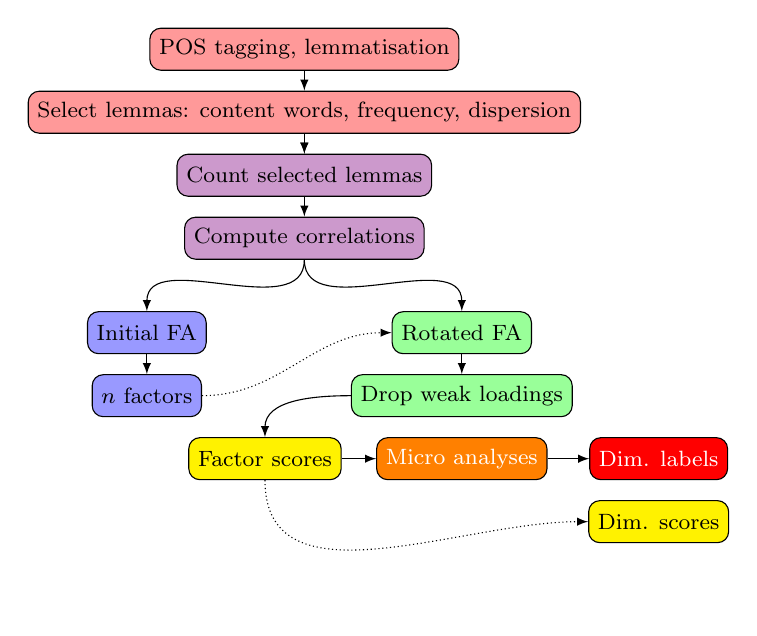
\begin{tikzpicture}
        %\tikzstyle{block} = [rectangle, rounded corners, text=black, text centered, draw=black, minimum height=.3in]
        \tikzstyle{block} = [rectangle, rounded corners, text=black, text centered, draw=black,font=\footnotesize, minimum height=.21in]
        \tikzstyle{line} = [-latex,draw=black,line width=.4]
        \node[block,fill=red!40,text=black] (tag) at (5,3) {POS tagging, lemmatisation};
        \node[block,fill=red!40,text=black] (key) at (5,2.2) {Select lemmas: content words, frequency, dispersion};
        \node[block,fill=violet!40,text=black] (binary) at (5,1.4) {Count selected lemmas};
        \node[block,fill=violet!40,text=black] (tetra) at (5,.6) {Compute correlations};
        \node[block,fill=blue!40,text=black] (fa1) at (3,-.6) {Initial FA};
        \node[block,fill=blue!40,text=black] (nfactors) at (3,-1.4) {$n$ factors};
        %\node[block,fill=blue!40,text=black] (comm) at (1,-.2) {Commun.};
        \node[block,fill=green!40,text=black] (fa2) at (7,-.6) {Rotated FA};
        \node[block,fill=green!40,text=black] (load) at (7,-1.4) {Drop weak loadings};
        %\node[block,fill=green!40,text=black] (standard) at (7,-1.6) {Standardise counts};
        \node[block,fill=yellow,text=black] (scores) at (4.5,-2.2) {Factor scores};
        \node[block,fill=orange,text=white] (analyse) at (7,-2.2) {Micro analyses};
        \node[block,fill=red,text=white] (labels) at (9.5,-2.2) {Dim. labels};
        \node[block,fill=yellow,text=black] (dimscores) at (9.5,-3) {Dim. scores};
        \draw[line] (tag) to (key);
        \draw[line] (key) to (binary);
        \draw[line] (key) to (binary);
        \draw[line] (binary) to (tetra);
        \draw[line] (fa1) to (nfactors);
        \draw[line] (tetra) to[in=90,out=270] (fa1);
        %\draw[line] (fa1) to (comm);
        \draw[line,densely dotted] (nfactors) to[in=180,out=0] (fa2);
        \draw[line] (tetra) to[in=90,out=270] (fa2);
        \draw[line] (fa2) to (load);
        %\draw[line] (load) to (standard);
        %\draw[line] (standard) to (scores);
        \draw[line] (load) to[in=90,out=180] (scores);
        \draw[line] (scores) to (analyse);
        \draw[line] (analyse) to (labels);
        \draw[line, densely dotted] (scores) to[in=180,out=270] (dimscores);
        %\draw[line,densely dashed] (standard) to (labels);
        %\draw[line,loosely dashed] (standard) to (labels);
    \end{tikzpicture}
    \caption{Lexical Multi-Dimensional Analysis Procedures}
    \label{fig:lexical_md_analysis_procedures}
\end{figure}
